\documentclass{standalone}


\usepackage{tikz}
\usetikzlibrary{arrows}

\begin{document}
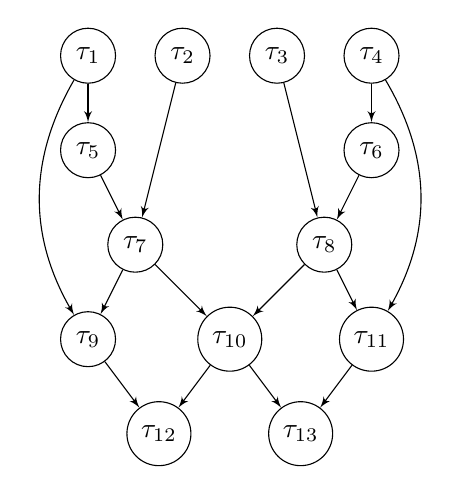
\begin{tikzpicture}[auto, node distance=1.2cm,>=latex']
\node[circle,draw] (t1) {$\tau_1$};
\node[circle,draw,right of = t1] (t2) {$\tau_2$};
\node[circle,draw,right of = t2] (t3) {$\tau_3$};
\node[circle,draw,right of = t3] (t4) {$\tau_4$};
\node[circle,draw,below of = t1] (t5) {$\tau_5$};
\node[circle,draw,below of = t4] (t6) {$\tau_6$};
\node[circle,draw,below of = t5,xshift=.6cm] (t7) {$\tau_7$};
\node[circle,draw,below of = t6,xshift=-.6cm] (t8) {$\tau_8$};
\node[circle,draw,below of = t7,xshift=-.6cm] (t9) {$\tau_9$};
\node[circle,draw,below of = t7,xshift=1.2cm] (t10) {$\tau_{10}$};
\node[circle,draw,below of = t8,xshift=.6cm] (t11) {$\tau_{11}$};
\node[circle,draw,below of = t10,xshift=-.9cm] (t12) {$\tau_{12}$};
\node[circle,draw,below of = t10,xshift=.9cm] (t13) {$\tau_{13}$};


\draw [->] (t1) -- (t5);
\draw [->] (t2) -- (t7);
\draw [->] (t3) -- (t8);
\draw [->] (t4) -- (t6);
\draw [->] (t5) -- (t7);
\draw [->] (t6) -- (t8);
\draw [->] (t7) -- (t9);
\draw [->] (t7) -- (t10);
\draw [->] (t8) -- (t10);
\draw [->] (t8) -- (t11);
\draw [->] (t10) -- (t12);
\draw [->] (t10) -- (t13);
\draw [->] (t9) -- (t12);
\draw [->] (t11) -- (t13);
\path (t4) edge[->,bend left] (t11);
\path (t1) edge[->,bend right] (t9);
    %
\end{tikzpicture}

\end{document}